\documentclass{article}
\usepackage[utf8]{inputenc}
\usepackage{hyperref}
\usepackage{listings}
\usepackage{xcolor}
\usepackage[margin=1in]{geometry}
\usepackage{booktabs}
\usepackage{longtable}
\usepackage{array}
\usepackage{enumitem}
\usepackage{fancyhdr}
\usepackage{titlesec}
\usepackage{tikz}
\usetikzlibrary{shapes.multipart, arrows.meta, positioning}

% --- Colour palette ------------------------------------------------------------
\definecolor{codegreen}{rgb}{0,0.6,0}
\definecolor{codegray}{rgb}{0.5,0.5,0.5}
\definecolor{codepurple}{rgb}{0.58,0,0.82}
\definecolor{backcolour}{rgb}{0.95,0.95,0.92}
\definecolor{evblue}{RGB}{30,100,200}
\definecolor{emsgreen}{RGB}{20,140,80}
\definecolor{rowgray}{gray}{0.92}

% --- Listing style -------------------------------------------------------------
\lstdefinestyle{mystyle}{
    backgroundcolor=\color{backcolour},
    commentstyle=\color{codegreen},
    keywordstyle=\color{magenta},
    numberstyle=\tiny\color{codegray},
    stringstyle=\color{codepurple},
    basicstyle=\ttfamily\footnotesize,
    breakatwhitespace=false,
    breaklines=true,
    captionpos=b,
    keepspaces=true,
    numbers=left,
    numbersep=5pt,
    showspaces=false,
    showstringspaces=false,
    showtabs=false,
    tabsize=2,
}
\lstdefinelanguage{json}{
    morestring=[b]",
    morecomment=[l]{//},
    sensitive=false,
}
\lstset{style=mystyle}

% --- HTTP method macros --------------------------------------------------------
\newcommand{\GET}{\colorbox{evblue!20}{\texttt{\textbf{\color{evblue}GET}}}}
\newcommand{\POST}{\colorbox{emsgreen!20}{\texttt{\textbf{\color{emsgreen}POST}}}}
\newcommand{\PUT}{\colorbox{emsgreen!35}{\texttt{\textbf{\color{emsgreen}PUT}}}}

% --- Page header ---------------------------------------------------------------
\pagestyle{fancy}
\fancyhf{}
\rhead{SIAM EV Platform --- EMS API (External)}
\lhead{\leftmark}
\rfoot{Page \thepage}
\renewcommand{\headrulewidth}{0.4pt}

\hypersetup{
    colorlinks=true,
    linkcolor=evblue,
    urlcolor=evblue,
    pdftitle={SIAM EV Platform - Energy Management System API Reference (External)},
    pdfauthor={Ruslee Sutthaweekul}
}

% --- Document ------------------------------------------------------------------
\title{%
    \textbf{SIAM EV Platform}\\[6pt]
    \large Energy Management System (EMS) API Reference\\
    \normalsize External Integration Edition
}
\author{Ruslee Sutthaweekul}
\date{Version 1.0 \quad\textbullet\quad \today}

\begin{document}

\maketitle
\tableofcontents
\newpage

% ==============================================================================
\section{Introduction}
% ==============================================================================

This document describes the REST and WebSocket APIs for the \textbf{Energy
Management System (EMS)} sub-system of the SIAM EV Unified Energy \& Logistics
Management Platform. It is a scoped extract of the full platform API reference,
prepared for handover to a development partner responsible for the EMS
facility/energy management system. It does not include the OCPP Charging
Monitoring or Cargo Space Monitoring APIs, which remain internal to SIAM EV; see
Section~\ref{sec:integration-notes} for what a partner integrator needs to know
about those boundaries.

The EMS sub-system aggregates energy consumption data from buildings and
facilities, provides time-series analytics, and exposes demand-response
controls. Data is persisted in TimescaleDB and read from SCADA / BMS systems
over Modbus TCP or MQTT.

A \emph{facility} is a physical site (office, retail, warehouse, or logistics
hub). A \emph{zone} is a named, bounded space inside a facility (cold room,
loading dock, dry-storage bay) with its own energy draw and environmental
sensors. EMS is the authoritative owner of all zone-level environmental and
energy sensor data on the platform.

\subsection{Base URL}

All endpoints are served under the API Gateway. Replace \texttt{\{host\}} with the
deployment address (e.g.\ \texttt{api.siam-ev.example.com}).

\begin{lstlisting}[language=bash, caption=Base URL pattern]
https://{host}/api/v1
\end{lstlisting}

\textbf{EMS base path:} \texttt{/api/v1/ems}

\subsection{Authentication}

Every request must carry a Bearer token obtained from the Auth Service.

\begin{lstlisting}[language=bash, caption=Authorization header]
Authorization: Bearer <access_token>
\end{lstlisting}

\begin{center}
\begin{tabular}{>{\ttfamily}lll}
\toprule
\textbf{Header} & \textbf{Required} & \textbf{Description}\\
\midrule
Authorization & Yes & \texttt{Bearer <JWT>} issued by \texttt{/auth/token}\\
Content-Type  & Yes (POST/PUT) & \texttt{application/json}\\
X-Request-ID  & No  & Idempotency key; echoed in response headers\\
\bottomrule
\end{tabular}
\end{center}

\subsection{Common Error Schema}

\begin{lstlisting}[language=json, caption=Error response envelope]
{
  "success": false,
  "error": {
    "code": "FACILITY_NOT_FOUND",
    "message": "No facility with id 'site-bkk-099' exists.",
    "timestamp": "2026-07-02T10:15:30Z"
  }
}
\end{lstlisting}

\begin{center}
\begin{tabular}{lll}
\toprule
\textbf{HTTP Status} & \textbf{Meaning} & \textbf{Common cause}\\
\midrule
200 & OK & Successful read\\
201 & Created & Resource created\\
400 & Bad Request & Missing or invalid fields\\
401 & Unauthorized & Missing / expired token\\
403 & Forbidden & Insufficient role\\
404 & Not Found & Resource does not exist\\
409 & Conflict & Duplicate resource\\
500 & Internal Error & Upstream / database failure\\
\bottomrule
\end{tabular}
\end{center}

\newpage

% ==============================================================================
\section{Data Models}
% ==============================================================================

\subsection{Object Model Overview}

\begin{figure}[h]
\centering
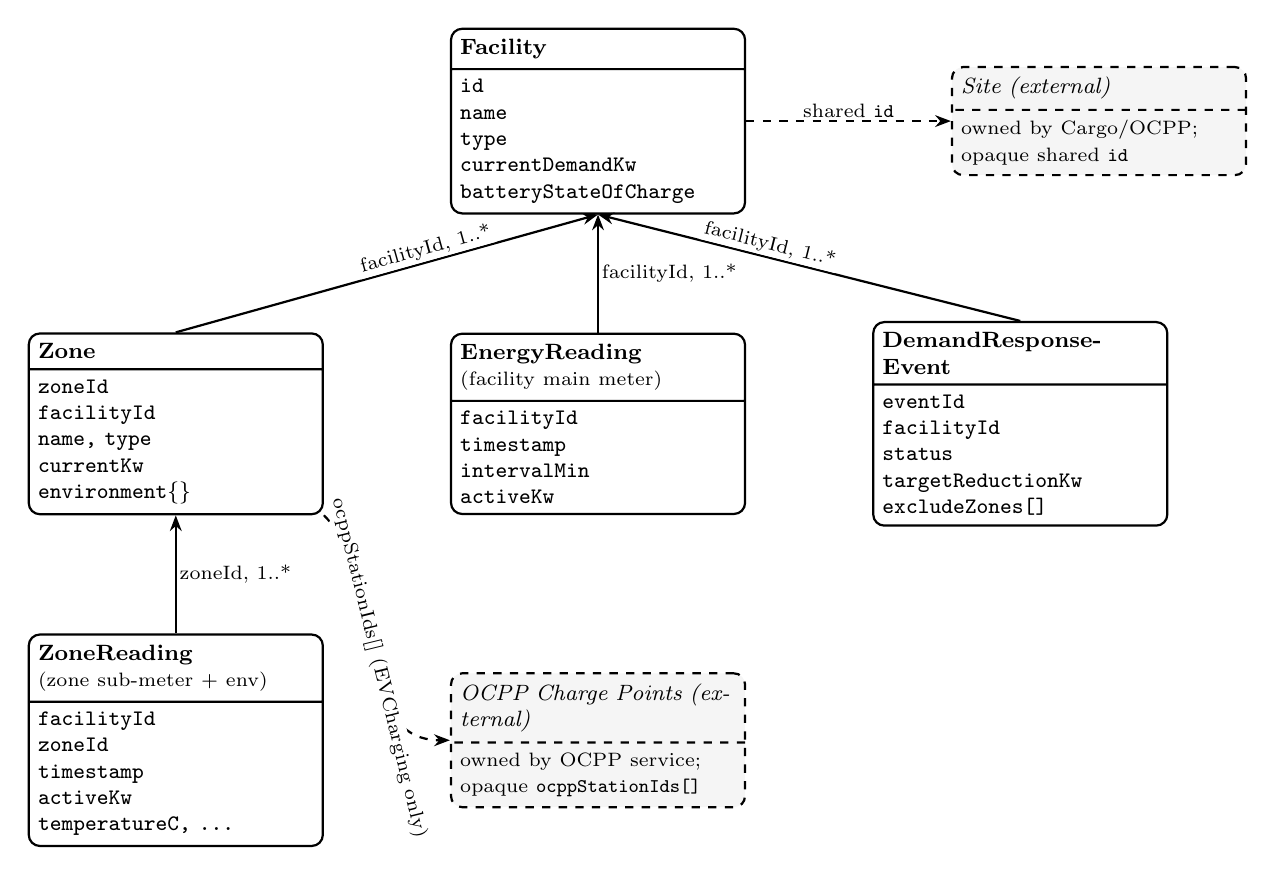
\begin{tikzpicture}[
    node distance=1.5cm and 1.6cm,
    class/.style={rectangle split, rectangle split parts=2, draw, thick,
                  rounded corners, rectangle split part align={center,left},
                  text width=3.5cm, font=\footnotesize},
    ext/.style={class, dashed, fill=gray!8},
    rel/.style={thick, -{Stealth[length=2mm]}},
    drel/.style={rel, dashed},
    lbl/.style={font=\scriptsize, fill=white, inner sep=1pt}
]

\node[class] (facility) {\textbf{Facility}
  \nodepart{second}\ttfamily id\\name\\type\\currentDemandKw\\batteryStateOfCharge};
\node[ext, right=2.6cm of facility] (site) {\textit{Site (external)}
  \nodepart{second}\scriptsize owned by Cargo/OCPP;\\opaque shared \texttt{id}};
\node[class, below=of facility] (reading) {\textbf{EnergyReading}\\\scriptsize(facility main meter)
  \nodepart{second}\ttfamily facilityId\\timestamp\\intervalMin\\activeKw};
\node[class, left=of reading] (zone) {\textbf{Zone}
  \nodepart{second}\ttfamily zoneId\\facilityId\\name, type\\currentKw\\environment\{\}};
\node[class, right=of reading] (dr) {\textbf{DemandResponse\-Event}
  \nodepart{second}\ttfamily eventId\\facilityId\\status\\targetReductionKw\\excludeZones[]};
\node[class, below=of zone] (zreading) {\textbf{ZoneReading}\\\scriptsize(zone sub-meter + env)
  \nodepart{second}\ttfamily facilityId\\zoneId\\timestamp\\activeKw\\temperatureC, ...};
\node[ext, right=of zreading] (ocpp) {\textit{OCPP Charge Points (external)}
  \nodepart{second}\scriptsize owned by OCPP service;\\opaque \texttt{ocppStationIds[]}};

\draw[drel] (facility.east) -- (site.west)
    node[lbl, above, pos=0.5] {shared \texttt{id}};
\draw[rel] (zone.north) -- (facility.south)
    node[lbl, above, sloped, pos=0.6] {facilityId, 1..*};
\draw[rel] (reading.north) -- (facility.south)
    node[lbl, right, pos=0.5] {facilityId, 1..*};
\draw[rel] (dr.north) -- (facility.south)
    node[lbl, above, sloped, pos=0.6] {facilityId, 1..*};
\draw[rel] (zreading.north) -- (zone.south)
    node[lbl, right, pos=0.5] {zoneId, 1..*};
\draw[drel] (zone.south east) to[out=-45, in=180]
    node[lbl, sloped, pos=0.55] {ocppStationIds[] (EVCharging only)} (ocpp.west);

\end{tikzpicture}
\caption{EMS object model --- solid arrows are foreign-key references within
this API. Note the two separate meter streams: \texttt{EnergyReading} is the
facility's main meter (keyed by \texttt{facilityId} only), while
\texttt{ZoneReading} is each zone's own sub-meter plus environment sensors
(keyed by \texttt{facilityId} \emph{and} \texttt{zoneId}) --- one does not
derive from the other.
\texttt{DemandResponseEvent.excludeZones[]} also references Zone by ID.
A \texttt{Zone} of \texttt{type: EVCharging} additionally references a group
of OCPP charge points via \texttt{ocppStationIds[]}. Dashed boxes mark data
whose owning system is out of scope for this document (see
Section~\ref{sec:integration-notes}).}
\end{figure}

\newpage

\subsection{Facility Object}

\begin{lstlisting}[language=json, caption=Facility object schema]
{
  "id":           "site-bkk-001",
  "name":         "Thai Post Sorting Hub --- Lad Krabang",
  "type":         "LogisticsWarehouse",  // Office | Retail | Warehouse | LogisticsWarehouse
  "location": {
    "lat": 13.7284,
    "lng": 100.7498,
    "address": "999 Moo 1, Lad Krabang, Bangkok 10520"
  },
  "ratedCapacityKva":    2000,
  "currentDemandKw":     312.4,
  "peakDemandKw":        1540.0,        // rolling 12-month peak
  "dailyEnergyKwh":      7820.5,
  "solarCapacityKw":     500,
  "batteryCapacityKwh":  1000,
  "batteryStateOfCharge": 0.78,         // 0.0--1.0
  "gridImportKw":        -45.2,         // negative = exporting to grid
  "demandResponseActive": false,
  "tariffZone":          "TOU-EV",
  "updatedAt": "2026-07-02T10:00:00Z"
}
\end{lstlisting}

\noindent\textbf{Note:} some facility IDs correspond to physical sites that are
also tracked by other internal SIAM EV systems (e.g.\ a logistics hub with its
own fleet operations). That correspondence is maintained internally and does
not appear in this schema; see Section~\ref{sec:integration-notes}.

\subsection{Zone Object (authoritative sensor record)}

A \emph{zone} is a named, bounded space inside a facility (cold room, loading
dock, dry-storage bay, EV charging area). All environmental sensor data for
zones is owned by EMS and read from the facility's BMS or SCADA system over
Modbus TCP or MQTT.

\begin{lstlisting}[language=json, caption=EMS zone object schema]
{
  "zoneId":      "zone-site-001-cold-01",
  "facilityId":  "site-bkk-001",
  "name":        "Cold Room A",
  "type":        "ColdRoom",    // ColdRoom | LoadingDock | DryBay | StagingArea | EVCharging
  // --- Energy (from SCADA / smart sub-meter) ---
  "currentKw":   42.1,
  "dailyKwh":    892.6,
  // --- Environment (from BMS sensors) ---
  "environment": {
    "temperatureC": 3.8,               // null if no temp sensor
    "humidityPct":  84.1,
    "co2Ppm":       405,
    "lightLux":     0
  },
  "setpointC":   4.0,                  // BMS setpoint (ColdRoom only)
  "thresholds": {
    "tempMinC":       2.0,
    "tempMaxC":       8.0,
    "humidityMaxPct": 90.0,
    "co2MaxPpm":      1000
  },
  "ocppStationIds": null,              // EVCharging only; see note below
  "alertActive": false,
  "source":      "BMS",                // BMS | SCADA | SmartMeter | Estimated
  "updatedAt":   "2026-07-02T10:02:00Z"
}
\end{lstlisting}

\begin{lstlisting}[language=json, caption=EMS zone object schema --- EVCharging zone example]
{
  "zoneId":      "zone-site-001-ev-01",
  "facilityId":  "site-bkk-001",
  "name":        "EV Charging Bay 1",
  "type":        "EVCharging",
  "currentKw":   96.4,                 // sum of the linked chargers' live draw
  "dailyKwh":    1204.7,
  "environment": { "temperatureC": null, "humidityPct": null, "co2Ppm": null, "lightLux": null },
  "setpointC":   null,
  "thresholds":  null,                 // EVCharging zones use OCPP-side limits, not BMS thresholds
  "ocppStationIds": ["station-bkk-001", "station-bkk-002"], // the EVSE group metered by this zone
  "alertActive": false,
  "source":      "SmartMeter",
  "updatedAt":   "2026-07-02T10:02:00Z"
}
\end{lstlisting}

\noindent\textbf{Note on \texttt{ocppStationIds}:} an \texttt{EVCharging} zone
groups a set of EVSEs/charge points for the purposes of sub-metering and
demand-response shedding; \texttt{currentKw} is the aggregate live draw of
that group. The station IDs themselves are opaque identifiers issued and
owned by the OCPP charging system, which is outside the scope of this
document --- treat them as strings for display/filtering and do not expect
to resolve charger-level detail (connector status, session state, etc.) from
the EMS API. See Section~\ref{sec:integration-notes}.

\subsection{Energy Reading Object (Time-Series) --- Facility Main Meter}

Keyed by \texttt{facilityId} only. This is the whole-site reading from the
facility's main incoming meter, returned by
\texttt{GET /ems/facilities/\{id\}/readings}.

\begin{lstlisting}[language=json, caption=Facility-level (main meter) energy reading schema]
{
  "facilityId":   "site-bkk-001",
  "timestamp":    "2026-07-02T10:00:00Z",
  "intervalMin":  15,                   // granularity of reading
  "activeKw":     315.2,
  "reactiveKvar": 42.1,
  "apparentKva":  317.9,
  "powerFactor":  0.991,
  "phaseA_V":     228.4,
  "phaseB_V":     229.1,
  "phaseC_V":     228.8,
  "source":       "SCADA"              // SCADA | BMS | SmartMeter | Estimated
}
\end{lstlisting}

\subsection{Zone Reading Object (Time-Series) --- Zone Sub-Meter}

Keyed by \texttt{facilityId} \emph{and} \texttt{zoneId}. This is a distinct
reading stream from the facility main meter above: each zone with its own
sub-meter or BMS sensor reports its own energy draw, combined with that
zone's environmental sensors in the same record. Returned by
\texttt{GET /ems/facilities/\{id\}/zones/\{zoneId\}/readings}.

\begin{lstlisting}[language=json, caption=Zone-level (sub-meter + environment) reading schema]
{
  "facilityId":   "site-bkk-001",
  "zoneId":       "zone-site-001-cold-01",
  "timestamp":    "2026-07-02T09:00:00Z",
  "intervalMin":  15,
  "activeKw":     44.8,                 // this zone's sub-meter, not the facility total
  "temperatureC": 3.9,
  "humidityPct":  85.2,
  "co2Ppm":       412
}
\end{lstlisting}

\noindent\textbf{Note:} a facility's main-meter \texttt{activeKw} is not simply
the sum of its zones' sub-meter readings --- common-area loads (lighting,
HVAC plant, office space) are metered only at the facility level and have no
corresponding zone.

\newpage

% ==============================================================================
\section{Facility Endpoints}
% ==============================================================================

\subsection{\GET\ \ \texttt{/ems/facilities} --- List facilities}

\textbf{Query parameters:}

\begin{center}
\begin{tabular}{>{\ttfamily}llll}
\toprule
\textbf{Param} & \textbf{Type} & \textbf{Default} & \textbf{Description}\\
\midrule
type    & string  & ---    & Filter by facility type\\
limit   & integer & 50   & Max records\\
offset  & integer & 0    & Pagination offset\\
\bottomrule
\end{tabular}
\end{center}

\textbf{Response 200:}
\begin{lstlisting}[language=json]
{
  "success": true,
  "data": [ /* array of Facility objects */ ],
  "meta": { "total": 8, "limit": 50, "offset": 0 }
}
\end{lstlisting}

\subsection{\GET\ \ \texttt{/ems/facilities/\{id\}} --- Get facility details}

Returns the latest live snapshot for a single facility.

\textbf{Response 200:}
\begin{lstlisting}[language=json]
{ "success": true, "data": { /* Facility object */ } }
\end{lstlisting}

\subsection{\GET\ \ \texttt{/ems/facilities/\{id\}/readings} --- Query time-series data}

Returns historical energy readings for a facility over a given time range.

\textbf{Query parameters:}

\begin{center}
\begin{tabular}{>{\ttfamily}llll}
\toprule
\textbf{Param} & \textbf{Type} & \textbf{Required} & \textbf{Description}\\
\midrule
from        & ISO-8601  & Yes  & Start of range (UTC)\\
to          & ISO-8601  & Yes  & End of range (UTC)\\
interval    & string    & No   & Bucket size: \texttt{15m} \textbar\ \texttt{1h} \textbar\ \texttt{1d} (default \texttt{15m})\\
metric      & string    & No   & Specific field to return (e.g.\ \texttt{activeKw})\\
\bottomrule
\end{tabular}
\end{center}

\textbf{Response 200:}
\begin{lstlisting}[language=json, caption=Time-series readings response]
{
  "success": true,
  "data": {
    "facilityId": "fac-bkk-001",
    "interval":   "1h",
    "readings": [
      { "timestamp": "2026-07-02T00:00:00Z", "activeKw": 180.4, "powerFactor": 0.98 },
      { "timestamp": "2026-07-02T01:00:00Z", "activeKw": 162.1, "powerFactor": 0.97 }
    ]
  }
}
\end{lstlisting}

\subsection{\GET\ \ \texttt{/ems/facilities/\{id\}/analytics} --- Demand analytics}

Returns aggregated KPIs for the facility over a billing period.

\textbf{Query parameters:} \texttt{period} --- \texttt{day} | \texttt{week} | \texttt{month} | \texttt{year} (default \texttt{month})

\textbf{Response 200:}
\begin{lstlisting}[language=json, caption=Analytics response]
{
  "success": true,
  "data": {
    "facilityId":         "fac-bkk-001",
    "period":             "month",
    "totalConsumptionKwh": 234156.2,
    "peakDemandKw":        1540.0,
    "peakTimestamp":       "2026-06-14T14:30:00Z",
    "avgLoadFactorPct":    42.8,
    "solarGenerationKwh":  31200.0,
    "selfConsumptionPct":  88.4,
    "gridImportKwh":       202956.2,
    "gridExportKwh":       3600.0,
    "estimatedCostThb":    812400.50,
    "carbonKgCo2e":        91188.0
  }
}
\end{lstlisting}

\subsection{\PUT\ \ \texttt{/ems/facilities/\{id\}/power-limit} --- Set import limit}

Caps the maximum grid import power draw for a facility.

\textbf{Request body:}
\begin{lstlisting}[language=json]
{
  "limitKw":    800,
  "reason":     "PeakDemandAvoidance",  // PeakDemandAvoidance | GridRequest | Manual
  "expiresAt":  "2026-07-02T16:00:00Z" // null = permanent until changed
}
\end{lstlisting}

\textbf{Response 200:}
\begin{lstlisting}[language=json]
{ "success": true, "data": { "facilityId": "fac-bkk-001", "limitKw": 800, "appliedAt": "..." } }
\end{lstlisting}

\subsection{\POST\ \ \texttt{/ems/facilities/\{id\}/demand-response} --- Trigger demand response}

Activates or deactivates a demand-response event for a facility (e.g.\ shed
non-critical loads to avoid peak demand charges).

\textbf{Request body:}
\begin{lstlisting}[language=json, caption=Demand-response command]
{
  "action":         "Activate",         // Activate | Deactivate
  "targetReductionKw": 200,             // required for Activate
  "durationMinutes":   30,              // required for Activate
  "priority":       "High",             // High | Medium | Low
  "notifyOccupants": true
}
\end{lstlisting}

\textbf{Response 200:}
\begin{lstlisting}[language=json]
{
  "success": true,
  "data": {
    "eventId":          "dr-20260702-001",
    "status":           "Activated",
    "activatedAt":      "2026-07-02T14:00:00Z",
    "expiresAt":        "2026-07-02T14:30:00Z",
    "projectedSavingKw": 195.3
  }
}
\end{lstlisting}

\noindent\textbf{Note:} the request body may optionally include an
\texttt{excludeZones} array of zone IDs to protect from shedding. Zone
protection decisions are made by SIAM EV's internal optimizer; the EMS system
only needs to honor whatever \texttt{excludeZones} list it receives.

\newpage

% ==============================================================================
\section{Zone Endpoints}
% ==============================================================================

\subsection{\GET\ \ \texttt{/ems/facilities/\{id\}/zones} --- List zones with sensor data}

Returns all zones within a facility with their current environmental readings
(temperature, humidity, CO\textsubscript{2}) and energy draw. This is the
\textbf{authoritative source} for zone sensor data on the platform.

\textbf{Response 200:}
\begin{lstlisting}[language=json, caption=Zone list with sensor and energy data]
{
  "success": true,
  "data": {
    "facilityId":     "site-bkk-001",
    "totalCurrentKw": 312.4,
    "zones": [
      {
        "zoneId":      "zone-site-001-cold-01",
        "name":        "Cold Room A",
        "type":        "ColdRoom",
        "currentKw":   42.1,
        "dailyKwh":    892.6,
        "environment": { "temperatureC": 3.8, "humidityPct": 84.1, "co2Ppm": 405 },
        "setpointC":   4.0,
        "alertActive": false
      },
      {
        "zoneId":    "zone-site-001-dock-03",
        "name":      "Loading Dock 3",
        "type":      "LoadingDock",
        "currentKw": 12.7,
        "dailyKwh":  84.3,
        "environment": { "temperatureC": 31.2, "humidityPct": 62.0, "co2Ppm": 510 },
        "alertActive": false
      },
      {
        "zoneId":    "zone-site-001-ev-01",
        "name":      "EV Charging Bay 1",
        "type":      "EVCharging",
        "currentKw": 96.4,
        "dailyKwh":  1204.7,
        "environment": { "temperatureC": null, "humidityPct": null, "co2Ppm": null },
        "ocppStationIds": ["station-bkk-001", "station-bkk-002"],
        "alertActive": false
      }
    ]
  }
}
\end{lstlisting}

\noindent\textbf{Note:} for some zone types, other internal SIAM EV systems may
associate additional operational context with a zone (e.g.\ dock occupancy,
or connector-level charging session detail for an \texttt{EVCharging} zone).
That context is not part of the EMS contract and is joined internally by
downstream consumers --- it does not need to be produced by this endpoint.

\subsection{\GET\ \ \texttt{/ems/facilities/\{id\}/zones/\{zoneId\}} --- Single zone detail}

Returns the full EMS Zone object for one zone, including the complete threshold
configuration and latest sensor readings.

\textbf{Response 200:}
\begin{lstlisting}[language=json]
{ "success": true, "data": { /* EMS Zone object */ } }
\end{lstlisting}

\subsection{\GET\ \ \texttt{/ems/facilities/\{id\}/zones/\{zoneId\}/readings} --- Zone sensor and energy history}

Returns time-series readings for a single zone, combining energy (kW) and
environmental sensors (temperature, humidity, CO\textsubscript{2}) in one
response. Accepts the same \texttt{from}/\texttt{to}/\texttt{interval}
parameters as the facility-level readings endpoint.

\textbf{Response 200:}
\begin{lstlisting}[language=json, caption=Zone sensor + energy time-series]
{
  "success": true,
  "data": {
    "facilityId": "site-bkk-001",
    "zoneId":     "zone-site-001-cold-01",
    "interval":   "1h",
    "readings": [
      { "timestamp": "2026-07-02T08:00:00Z",
        "activeKw": 40.2, "temperatureC": 4.1, "humidityPct": 83.5, "co2Ppm": 398 },
      { "timestamp": "2026-07-02T09:00:00Z",
        "activeKw": 44.8, "temperatureC": 3.9, "humidityPct": 85.2, "co2Ppm": 412 }
    ]
  }
}
\end{lstlisting}

\subsection{\PUT\ \ \texttt{/ems/facilities/\{id\}/zones/\{zoneId\}/thresholds} --- Update zone thresholds}

Sets the alert thresholds for a zone. Alerts from this endpoint surface on the
EMS WebSocket (\texttt{AlertTriggered}) and may also be surfaced to other
internal SIAM EV dashboards; that distribution is handled internally and
requires no action from the EMS system beyond emitting the WebSocket event.

\textbf{Request body:}
\begin{lstlisting}[language=json]
{
  "tempMinC":       2.0,
  "tempMaxC":       8.0,
  "humidityMaxPct": 90.0,
  "co2MaxPpm":      1000
}
\end{lstlisting}

\textbf{Response 200:}
\begin{lstlisting}[language=json]
{ "success": true, "data": { "zoneId": "zone-site-001-cold-01", "thresholds": { ... } } }
\end{lstlisting}

\newpage

% ==============================================================================
\section{WebSocket --- Live Energy Feed}
% ==============================================================================

\begin{lstlisting}[language=bash]
wss://{host}/api/v1/ems/ws?facilityId=fac-bkk-001&token=<access_token>
\end{lstlisting}

\textbf{Server-sent event frame:}
\begin{lstlisting}[language=json, caption=EMS live push event]
{
  "event":      "EnergyReading",
  "facilityId": "fac-bkk-001",
  "data": {
    "activeKw":     318.7,
    "solarKw":       52.1,
    "batteryKw":    -10.0,    // negative = discharging (exporting to facility)
    "gridKw":       276.6,
    "soc":           0.74,
    "timestamp":    "2026-07-02T10:05:00Z"
  }
}
\end{lstlisting}

\begin{center}
\begin{tabular}{ll}
\toprule
\textbf{event} & \textbf{Trigger}\\
\midrule
\texttt{EnergyReading}     & Every 15 s from SCADA/BMS poller\\
\texttt{DemandAlert}       & Demand approaches \textgreater 90\% of contract capacity\\
\texttt{SolarForecast}     & Hourly PV generation forecast update\\
\texttt{BatteryStateChange}& SoC crosses 20\%, 50\%, or 80\% threshold\\
\texttt{DemandResponseEvent}& DR event activated or deactivated\\
\texttt{AlertTriggered}    & Zone threshold breach (see zone thresholds endpoint)\\
\texttt{AlertResolved}     & Zone reading returns within threshold\\
\bottomrule
\end{tabular}
\end{center}

\newpage

% ==============================================================================
\section{Integration Notes}
\label{sec:integration-notes}
% ==============================================================================

This section summarizes, at a high level, how EMS fits into the wider SIAM EV
platform. Details of the other sub-systems are intentionally excluded from
this handover document.

\begin{itemize}[leftmargin=*]
    \item \textbf{Facility identity is shared internally.} A \texttt{facilityId}
          (e.g.\ \texttt{site-bkk-001}) may correspond to the same physical site
          in other internal SIAM EV systems (e.g.\ a logistics hub tracked by a
          separate fleet-management system). This cross-reference is coordinated
          entirely on the SIAM EV side; the EMS API contract in this document
          does not change based on it, and no additional integration work is
          required by the EMS system to support it.
    \item \textbf{Zone protection during demand response.} SIAM EV's internal
          optimizer may ask EMS to exclude specific zones from a shed event via
          the \texttt{excludeZones} field on \texttt{POST
          /ems/facilities/\{id\}/demand-response}. The EMS system does not need
          to know why a zone is protected --- only to honor the list it receives.
    \item \textbf{Smart charging coordination.} SIAM EV may adjust EV charger
          power limits in response to EMS demand alerts. This coordination is
          performed by an internal optimizer that consumes the EMS WebSocket
          feed and calls \texttt{PUT /ems/facilities/\{id\}/power-limit} to
          register the applied cap; it requires no changes to the EMS API.
    \item \textbf{\texttt{EVCharging} zones reference a group of OCPP charge
          points.} A zone of \texttt{type: "EVCharging"} carries an
          \texttt{ocppStationIds[]} array (see the Zone Object schema) so that
          the zone's aggregate \texttt{currentKw} can be reconciled against
          the underlying chargers by SIAM EV's internal systems. The EMS
          system only needs to store and return this array as opaque strings
          --- it does not call the OCPP API, does not need to validate the
          IDs, and does not need connector-level detail (session state,
          connector status, etc.); that detail lives entirely in the OCPP
          charging system, which is out of scope for this document.
    \item \textbf{Out of scope for this handover.} OCPP charging telemetry, the
          Cargo Space Monitoring API, and the outbound webhook registry are
          separate SIAM EV--internal systems and are not included here. If a
          future feature requires the EMS system to call one of those APIs
          directly, SIAM EV will provide a supplementary interface
          specification at that time.
\end{itemize}

\newpage

% ==============================================================================
\section{API Quick Reference}
% ==============================================================================

\begin{longtable}{>{\ttfamily\footnotesize}p{0.45\textwidth} p{0.08\textwidth} p{0.38\textwidth}}
\toprule
\textbf{Endpoint} & \textbf{Method} & \textbf{Description}\\
\midrule
\endfirsthead
\toprule
\textbf{Endpoint} & \textbf{Method} & \textbf{Description}\\
\midrule
\endhead
\bottomrule
\endfoot

\multicolumn{3}{l}{\textit{Facilities}}\\[2pt]
/ems/facilities                     & GET    & List facilities\\
/ems/facilities/\{id\}              & GET    & Facility live snapshot\\
/ems/facilities/\{id\}/readings     & GET    & Time-series energy readings\\
/ems/facilities/\{id\}/analytics    & GET    & Demand KPIs for billing period\\
/ems/facilities/\{id\}/demand-response     & POST & Activate / deactivate DR event\\
/ems/facilities/\{id\}/power-limit         & PUT  & Cap grid import power\\[4pt]

\multicolumn{3}{l}{\textit{Zones}}\\[2pt]
/ems/facilities/\{id\}/zones               & GET  & All zones: sensor + energy data (authoritative)\\
/ems/facilities/\{id\}/zones/\{zoneId\}   & GET  & Single zone detail\\
/ems/facilities/\{id\}/zones/\{zoneId\}/readings & GET & Zone sensor + energy time-series\\
/ems/facilities/\{id\}/zones/\{zoneId\}/thresholds & PUT & Update zone alert thresholds\\[4pt]

\multicolumn{3}{l}{\textit{WebSocket}}\\[2pt]
/ems/ws                                    & WS   & Live energy feed\\
\end{longtable}

\end{document}
